%! TeX root = /Users/trustinnguyen/Downloads/Berkeley/Math/Math128a/Homework/Math128aHw1.tex

\documentclass{article}
\usepackage{/Users/trustinnguyen/.mystyle/math/packages/mypackages}
\usepackage{/Users/trustinnguyen/.mystyle/math/commands/mycommands}
\usepackage{/Users/trustinnguyen/.mystyle/math/environments/article}
\graphicspath{{./figures/}}

\title{Math128aHw1}
\author{Trustin Nguyen}

\begin{document}

    \maketitle

\section*{Section 1.1}
\hrule
\textbf{Exercise 2}:
    Show that the following equations have at least one solution in the given intervals.
    \begin{itemize}
        \item [(c)] $-3\tan(2x) + x = 0, \, [0, 1]$
            \begin{answer}
               Observe that plugging in $0$, we get:
                    \begin{equation*}
                        -3\tan(0) + 0 = 0 + 0 = 0
                    \end{equation*}
                as desired.
            \end{answer}

        \item [(d)] $\ln(x) - x^{2} + \frac{5}{2}x - 1, \, [\frac{1}{2}, 1]$
            \begin{answer}
                We plug in $\frac{1}{2}$ to get:
                    \begin{equation*}
                        \ln(\frac{1}{2}) - \left(\frac{1}{2}\right)^2 + \frac{5}{4} - 1 = \ln(\frac{1}{2}) + 2 - 1 = \ln(\frac{1}{2}) - 1 < 0
                    \end{equation*}
                Now plug in $1$:
                    \begin{equation*}
                        \ln(1) - 1 + \frac{5}{2} - 1 = 0 - 2 + \frac{5}{2} > 0
                    \end{equation*}
                Because $f(x) = \ln{x} - x^2 + \frac{5}{2}x - 1$ is a continuous function on the interval $[\frac{1}{2}, 1]$, we know that by the intermediate value theorem, there is an $x \in [\frac{1}{2}, 1]$ such that $f(x) = 0$
            \end{answer}
    \end{itemize}

\textbf{Exercise 4}:
    Find intervals containing solutions to the following equations.
    \begin{itemize}
        \item [(d)] $x^3 + 4.001x^2 + 4.002x + 1.101 = 0$.
        \begin{answer}
            Taking the derivative, we get $3x^2 + 4.001x + 4.002$. The determinant
                \begin{equation*}
                    b^{2} - 4ac = 4.001^{2} - 4 * 4.002 * 3 < 0
                \end{equation*}
            This means the graph is strictly increasing, there is one solution. If we plug in $-4$ and $0$, we get:
                \begin{equation*}
                    -4^{3} + 4.001 * (-4)^{2} + 4.002(-4) + 1.101 < 0
                \end{equation*}
            So an interval with the solution is $[-4, 0]$.
        \end{answer}
    \end{itemize}

\textbf{Exercise 6}:
    Find $\max_{a \leq x \leq b}(\lvert f(x) \rvert)$ for the following functions and intervals.
    \begin{itemize}
        \item [(a)] $f(x) = 2x / (x^{2} + 1), \, [0, 2]$.
            \begin{answer}
                Find the derivative:
                    \begin{equation*}
                        f^{\prime}(x) = \dfrac{2x^{2} + 2 - 4x^{2}}{(x^{2} + 1)^{2}} = \dfrac{-2(x^{2} - 1)}{x^{4} + 2x^{2} + 1}
                    \end{equation*}
                The function is negative when $-2(x^{2} - 1) < 0$ or when $x > 1, x < -1$. This means that $f(x)$ is increasing on $[0, 1]$, decreasing on $[1, 2]$. So the max is at $x = 1$, $f(1) = 2 / 2 = 1$
            \end{answer}
    \end{itemize}

\textbf{Exercise 14}:
    Let $f(x) = 2x\cos{2x} - (x - 2)^{2}$ and $x_{0} = 0$.
        \begin{itemize}
            \item [(a)] Find the third Taylor polynomial $P_{3}(x)$ and use it to approximate $f(0.4)$.
                \begin{answer}
                    $f(0) = 0 - 4 = -4$, \\
                    $f^{\prime}(x) = 2 \cos{2x} - 4x \sin{2x} - 2(x - 2), \, f^{\prime}(0) = 6$, \\
                    $f^{\prime\prime}(x) = - 8 \sin{2x} - 8x \cos{2x} - 2, \, f^{\prime\prime}(0) = -2$ \\
         S           $f^{\prime\prime\prime}(x) = -24 \cos{2x} + 16x \sin{2x}, \, f^{\prime\prime\prime}(0) = -24$ \\
                    So the polynomial is $P_{3}(x) = -4x^{3} -x^{2} + 6x - 4$
                \end{answer}

            \item [(b)] Use the error formula in Taylor's Theorem to find an upper bound for the error $\lvert f(0.4) - P_{3}(0.4) \rvert$. Compute the actual error.
                \begin{answer}
                    The error is given my the next term:
                        \begin{equation*}
                            \left\lvert \dfrac{f^{4}(\varepsilon(x))}{4!} x^{4} \right\rvert
                        \end{equation*}
                    The next derivative is:
                        \begin{equation*}
                            f^{(4)} = 64 \sin{ 2x} + 32x \cos{2x} 
                        \end{equation*}
                    So the error is $(\frac{8}{3} \sin{2\varepsilon(x)} + \frac{4}{3}\varepsilon(x) \cos{2\varepsilon(x)})x^{4}$. Since $0 \leq \varepsilon(x) \leq 0.4$, we just compute the max of the function on that interval.
                    Taking the derivative, we get:
                        \begin{equation*}
                            \dfrac{20}{3} \cos{2x} - \dfrac{8}{3} x\sin{2x}
                        \end{equation*}
                    It is easy to see that this function is positive on the interval because $\cos{2x} > .5$ on the interval and $\sin{2x} < 1$ on the interval. So $x \sin{ 2x} < .4$, and it follows:
                        \begin{equation*}
                            .5 * \dfrac{20}{3} - \dfrac{8}{3} .4 > 0
                        \end{equation*}
                    So the max error is $(.4)^{4}(\frac{8}{3} \sin{.8} + \frac{4}{3}* .4 \cos{.8})$. The actual error can be obtained by plugging in the numbers:
                        \begin{equation*}
                            \left\lvert .8 \cos{.8} - (1.8)^{2} - (-4(.4)^{3} - (.4)^{2} + 6(.4) - 4) \right\rvert
                        \end{equation*}
                \end{answer}

            \item [(c)] Find the fourth Taylor polynomial $P_{4}(x)$ and use it to approximate $f(0.4)$.
                \begin{answer}
                    The fourth derivative was calculated in the previous part:
                        \begin{equation*}
                            f^{(4)}(x) = 64 \sin{2x} + 32x \cos{2x}
                        \end{equation*}
                    so $f^{4}(0) = 0$ and $P_{4}(x) = -4x^{3} - x^{2} + 6x - 4$. Then the approximation of $f(0.4)$ is $-4(.4)^{3} - (0.4)^{2} + 6(0.4) - 4$.
                \end{answer}

            \item [(d)] Use the error formula in Taylor's Theorem to find an upper bound for the error $\lvert f(0.4) - P_{4}(0.4) \rvert$. Compute the actual error. 
                \begin{answer}
                    This is the error as part $b$ because $P_{3}(x) = P_{4}(x)$. The upper bound would be a little different. Calculate the derivative of 
                        \begin{equation*}
                            f^{(4)}(x) = 64 \sin{2x} + 32x \cos{2x}
                        \end{equation*}
                    which is
                        \begin{equation*}
                            f^{(5)}(x) = 160 \cos{2x} - 64x \sin{2x}
                        \end{equation*}
                    So we have to find the max of 
                        \begin{equation*}
                            \lvert 160 \cos{2 \varepsilon(x)} - 64 \varepsilon(x) \sin{2 \varepsilon(x)} \rvert (0.4)^{5} / 5!
                        \end{equation*}
                    in the interval $[0, 0.4]$. Taking the derivative:
                        \begin{equation*}
                            -384 \sin{2x} - 64x \cos{2x}
                        \end{equation*}
                    This is clearly $< 0$ on the interval, so the max is at $\varepsilon(x) = 0$. This gives the max error of $160 * (0.4)^{5} / 5! = 4 * (0.4)^{5} / 3$ 
                \end{answer}
        \end{itemize}

\textbf{Exercise 26}:
    Prove the Generalized Rolle's Theorem, Theorem 1.10, by verifying the following.
    \begin{itemize}
        \item [(a)] Use Rolle's Theorem to show that $f^{\prime}(z_{i}) = 0$ for $n - 1$ numbers in $[a, b]$ with $a \leq z_{1} < z_{2} < \cdots < z_{n - 1} \leq b$.
            \begin{answer}
                Suppose that $f \in C[a, b]$ is $n - 1$ times differentiable on $(a, b)$ and that $f(x) = 0$ at $n$ distinct points $a < z_{1} < z_{2} < \cdots < z_{n - 1} < b$. Then we can apply Rolle's theorem to each interval $(z_{1}, z_{2}), (z_{2}, z_{3}), \ldots, (z_{n - 2}, z_{n - 1})$. Since $f(z_{i}) = f(z_{i + 1})$, by Rolle's theorem there are $n - 1$ distinct $x$ such that $f^{\prime}(x) = 0$.
            \end{answer}

        \item [(b)] Use Rolle's Theorem to show that $f^{(2)}(w_{i}) = 0$ for $n - 2$ numbers in $[a, b]$ with $z_{1} < w_{1} < z_{2} < w_{2} < \cdots < w_{n - 2} < z_{n - 1} < b$.
            \begin{answer}
                We have that $f^{\prime}(z_{i}) = 0$. We apply Rolle's Theorem to the intervals $(z_{1}, z_{2}), (z_{2}, z_{3}), \ldots, (z_{n - 2}, z_{n - 1})$. Since $f^{\prime}(z_{i}) = f^{\prime}(z_{i + 1})$, by the theorem, there exists $z_{i} < w_{i} < z_{i + 1}$ such that $f^{\prime\prime}(w_{i}) = 0$. Repeated for all intervals, we have at least $n - 2$ unique roots for $f^{\prime\prime}$ on the interval $(a, b)$
            \end{answer}

        \item [(c)] Continue the arguments in parts (a) and (b) to show that for each $j = 1, 2, \ldots, n - 1$, there are $n - j$ distinct numbers in $[a, b]$, where $f^{(j)}$ is $0$.
            \begin{answer}
                Base case: $j = 1$. Done in part $a$.

                Inductive case: Suppose that this is true for $j = i$. We will prove this holds for $i + 1 < n - 1$.

                Since there are $n - i$ values in the interval $a < w_{1} < w_{2} < \cdots < w_{n - i} < b$ such that $f^{(i)}(w_{k}) = 0$, we apply Rolle's Theorem to the intervals $(w_{1}, w_{2}), (w_{2}, w_{3}), \ldots, (w_{n - i - 1}, w_{n - i})$ to get $n - i - 1 = n - (i + 1)$ values $a < w_{1} < q_{1} < w_{2} < q_{2} < \cdots < q_{n - i - 2} < w_{n - i - 1} < q_{n - i - 1} < w_{n - i}$ where $f^{i + 1}(q_{k}) = 0$. So we are done.
            \end{answer}

        \item [(d)] Show that part (c) implies the conclusion of the theorem.
            \begin{answer}
                Part $c$ tells us that when $j = n - 1$, then there is $1$ distinct numbers in $[a, b]$ where $f^{(n - 1)}(q) = 0$. This is the statement for Rolle's Theorem for when $f$ is differentiable $n - 1$ times.
            \end{answer}
    \end{itemize}

\newpage
\section*{Section 1.2}
\hrule

\textbf{Exercise 2}:
    Compute the absolute error and relative error in approximations of $p$ by $p^{*}$.
        \begin{itemize}
            \item [(c)] $p = 8!, p^{*} = 39900$ 
                \begin{answer}
                    We have $p = 40320$. The absolute error is $p - p^{*} = 420$. The absolute error is $\lvert p - p^{*} \rvert / \lvert p \rvert = 0.010416666666667$.
                \end{answer}
        \end{itemize}

\textbf{Exercise 4}:
    Find the largest interval in which $p^{*}$ must lie to approximate $p$ with relative error at most $10^{-4}$ for each value of $p$.
        \begin{itemize}
            \item [(b)] $e$
                \begin{answer}
                    We have an interval of the form $[e - \delta, e + \delta]$ and such that $\lvert e - p^{*} \rvert / e \leq 10^{-4}$. If $e \geq p^{*}$,
                        \begin{equation*}
                            e - p^{*} \leq e * 10^{-4}
                        \end{equation*}
                    which means the lower bound is $e(1 - 10^{-4})$. If $e \leq p^{*}$, then 
                        \begin{equation*}
                            p^{*} - e \leq e * 10^{-4}
                        \end{equation*}
                    which means the upper bound is $e(1 + 10^{-4})$. So the interval is $[e(1 - 10^{-4}), e(1 + 10^{-4})]$. 
                \end{answer}
        \end{itemize}

\textbf{Exercise 12}:
    The number $e$ can be defined by $e = \sum_{n = 0}^{\infty}(1 / n!)$, where $n! = n(n - 1) \cdots 2 \cdot 1$ for $n \neq 0$ and $0! = 1$. Compute the absolute error and relative error in approximations of $e$:
        \begin{itemize}
            \item [(a)] $\sum_{n = 0}^{5} \frac{1}{n!}$
                \begin{answer}
                    The absolute error is $\sum_{n = 0}^{\infty} (1 / n!) - \sum_{n = 0}^{5} (1 / n!) = \exp(1) - (1 + 1 + (1 / 2) + (1 / 6) + (1 / 24)) = \exp(1) - 2.7083333333333 = 0.00994849512574$. The relative error is $0.00994849512574 / \exp(1) = 0.00365984682735$
                \end{answer}

            \item [(b)] $\sum_{n = 0}^{10} \frac{1}{n!}$ 
                \begin{answer}
                    The absolute error is $\sum_{n = 0}^{\infty} (1 / n!) - \sum_{n = 0}^{10} (1 / n!)$ which is 
                        \begin{equation*}
                            \exp(1) - (1 + 1 + (1 / 2) + (1 / 6) + (1 / 24) + (1 / 120) + (1 / 720) + (1 / 5040) + (1 / 40320) + (1 / 362880) + (1 / 3628800))
                        \end{equation*}
                    where $(1 + 1 + (1 / 2) + (1 / 6) + (1 / 24) + (1 / 120) + (1 / 720) + (1 / 5040) + (1 / 40320) + (1 / 362880) + (1 / 3628800)) = 2.7182818011464$. Then the absolute error is $\exp(1) - 2.7182818011464 = 2.73126450345e-8$. The relative error is then $2.73126450345e-8 / \exp(1) = 9.1042150115e-9$
                \end{answer}
        \end{itemize}

\textbf{Exercise 22}:
    The Taylor polynomial for $f(x) = e^{x}$ is $\sum_{i = 0}^{n}(x^{i} / i!)$. Use the Taylor polynomial of degree nine and three-digit chopping arithmetic to find an approximation to $e^{-5}$ by each of the following methods.
        \begin{itemize}
            \item [(a)] $e^{-5} \approx \sum_{i = 0}^{9} \frac{(-5)^{i}}{i!} = \sum_{i = 0}^{9} \frac{(-1)^{i}5^{i}}{i!}$ 
                \begin{answer}
                    We have that 
                        \begin{equation*}
                            \sum_{i = 0}^{9} \dfrac{(-1)^{i}5^{i}}{i!} = -1.82710537919 = -.182710537919 \times 10^{1} \rightarrow -0.182 \times 10^{1}
                        \end{equation*}
                \end{answer}

            \item [(b)] $e^{-5} = \frac{1}{e^{5}} \approx \frac{1}{\sum_{i = 0}^{9} \frac{ 5^{i}}{i!}}$
                \begin{answer}
                    We have 
                        \begin{equation*}
                            \dfrac{1}{\sum_{i = 0}^{9}\frac{5^{i}}{i!}} = 0.00695945286365 = 0.657452463635 \times 10^{-2} \rightarrow 0.657 \times 10^{-2}
                        \end{equation*}
                \end{answer}

            \item [(c)] An approximate value of $e^{-5}$ correct to three digits is $6.74 \times 10^{-3}$. Which formula, $(a)$ or $(b)$, gives the most accuracy, and why? 
                \begin{answer}
                    For $e^{-5}$,
                        \begin{equation*}
                            e^{-5} = 0.00673794699909 = 0.673794699909 \times 10^{-2} \rightarrow 0.673 \times  10^{-2}
                        \end{equation*}
                    Method $b$ is more accurate
                \end{answer}
        \end{itemize}

\newpage
\section*{Section 1.3}
\hrule

\textbf{Exercise 8}:
    Suppose that $0 < q < p$ and that $\alpha_{n} = \alpha + \mathcal{O}(n^{-p})$.
        \begin{itemize}
            \item [(a)] Show that $\alpha_{n} = \alpha + \mathcal{O}(n^{-q})$.
                \begin{answer}
                    Since $\alpha_{n} = \alpha + \mathcal{O}(n^{-p})$, we know that the convergence of $\alpha_{n}$ is bounded by that of $n^{-p}$:
                        \begin{equation*}
                            \lvert \alpha_{n} - \alpha \rvert \leq k\lvert n^{-p} \rvert
                        \end{equation*}
                    Since $q < p$, we know that:
                        \begin{equation*}
                            \lvert n^{q} \rvert < \lvert n^{p} \rvert \implies \lvert n^{-p} \rvert < \lvert n^{-q} \rvert
                        \end{equation*}
                    putting this in our previous equation, we get:
                        \begin{equation*}
                            \lvert \alpha_{n} - \alpha \rvert \leq k \lvert n^{-p} \rvert < k \lvert n^{-q} \rvert
                        \end{equation*}
                    and therefore, $\alpha_{n} = \alpha + \mathcal{O}(n^{-q})$.
                \end{answer}

            \item [(b)] Make a table listing $1/n, 1/n^{2}, 1/n^{3}, $ and $1/n^{4}$ for $n = 5, 10, 100, $ and $1000$ and discuss varying rates of convergence of these sequences as $n$ becomes large. 
                \begin{answer}
                    Table:
                        \begin{align*}
                            \begin{array}{ c c c c c }
                                         & 1/n    & 1/n^{2}    & 1/n^{3}      & 1/n^{4}         \\
                                n = 5    & 1/5    & 1/25       & 1/125        & 1/625           \\
                                n = 10   & 1/10   & 1/100      & 1/1000       & 1/1000          \\
                                n = 100  & 1/100  & 1/10000    & 1/1000000    & 1/1000000       \\
                                n = 1000 & 1/1000 & 1/10000000 & 1/1000000000 & 1/1000000000000   
                            \end{array}
                        \end{align*}
                    As $n$ becomes large, the sequences with higher exponent in the denominator converge faster.
                \end{answer}
        \end{itemize}

\textbf{Exercise 15}:
    \begin{itemize}
        \item [(a)] How many multiplications and additions are required to determine a sum of the form 
            \begin{equation*}
                \sum_{i = 1}^{n} \sum_{j = 1}^{i}a_{i}b_{j}?
            \end{equation*}
            \begin{answer}
                The number of multiplications is $1 + 2 + 3 + 4 + \cdots + n$. This gives us $n(n + 1) / 2$ multiplications. The number of additions is $(n(n + 1) / 2) - 1$ because there are $n(n + 1) / 2$ terms after multiplication.
            \end{answer}

        \item [(b)] Modify the sum in part $(a)$ to an equivalent form that reduces the number of computations. 
            \begin{answer}
                We can pull the $a_{i}$ out:
                    \begin{equation*}
                        \sum_{i = 1}^{n}a_{i}\sum_{j = 1}^{i}b_{j}
                    \end{equation*}
                This gives us $n$ multiplications and $n + (0 + 1 + 2 + \cdots n - 1)$ additions, or just $1 + 2 + \cdots n = (n + 1)n / 2$ additions.
            \end{answer}
    \end{itemize}

\textbf{Exercise 2}:
    Construct an algorithm that has as input an integer $n \geq 1$, numbers $x_{0}, x_{1}, \ldots, x_{n}$, and a number $x$ and that produces as output the product $(x - x_{0})(x - x_{1}) \cdots (x - x_{n})$.
        \begin{answer}
            Algorithm:
            \begin{center}
                def f(roots, x): \\
                \hspace{5cm} return prod([(x - r) for r in roots])
            \end{center}
        \end{answer}

\newpage
\section*{Section 2.1}
\hrule

\textbf{Exercise 6}:
    Use the Bisection method to find solutions, accurate to within $10^{-5}$ for the following problems.
    \begin{itemize}
        \item [(d)] $x + 1 - 2\sin{\pi x} = 0$ for $0 \leq x \leq 0.5$ and $0.5 \leq x \leq 1$.
    \end{itemize}
    \begin{answer}
        Here is my bisection.m file:
        \inputminted{matlab}{bisection.m}
        And my function:
        \inputminted{matlab}{myfunc.m}
        And the script that is ran:
        \inputminted{matlab}{script.m}
        The output given is $x = 0.206035614013671875$.
    \end{answer}

\textbf{Exercise 8}:
    \begin{itemize}
        \item [(a)] Sketch the graphs of $y = x$ and $y = \tan{x}$.
            \begin{center}
                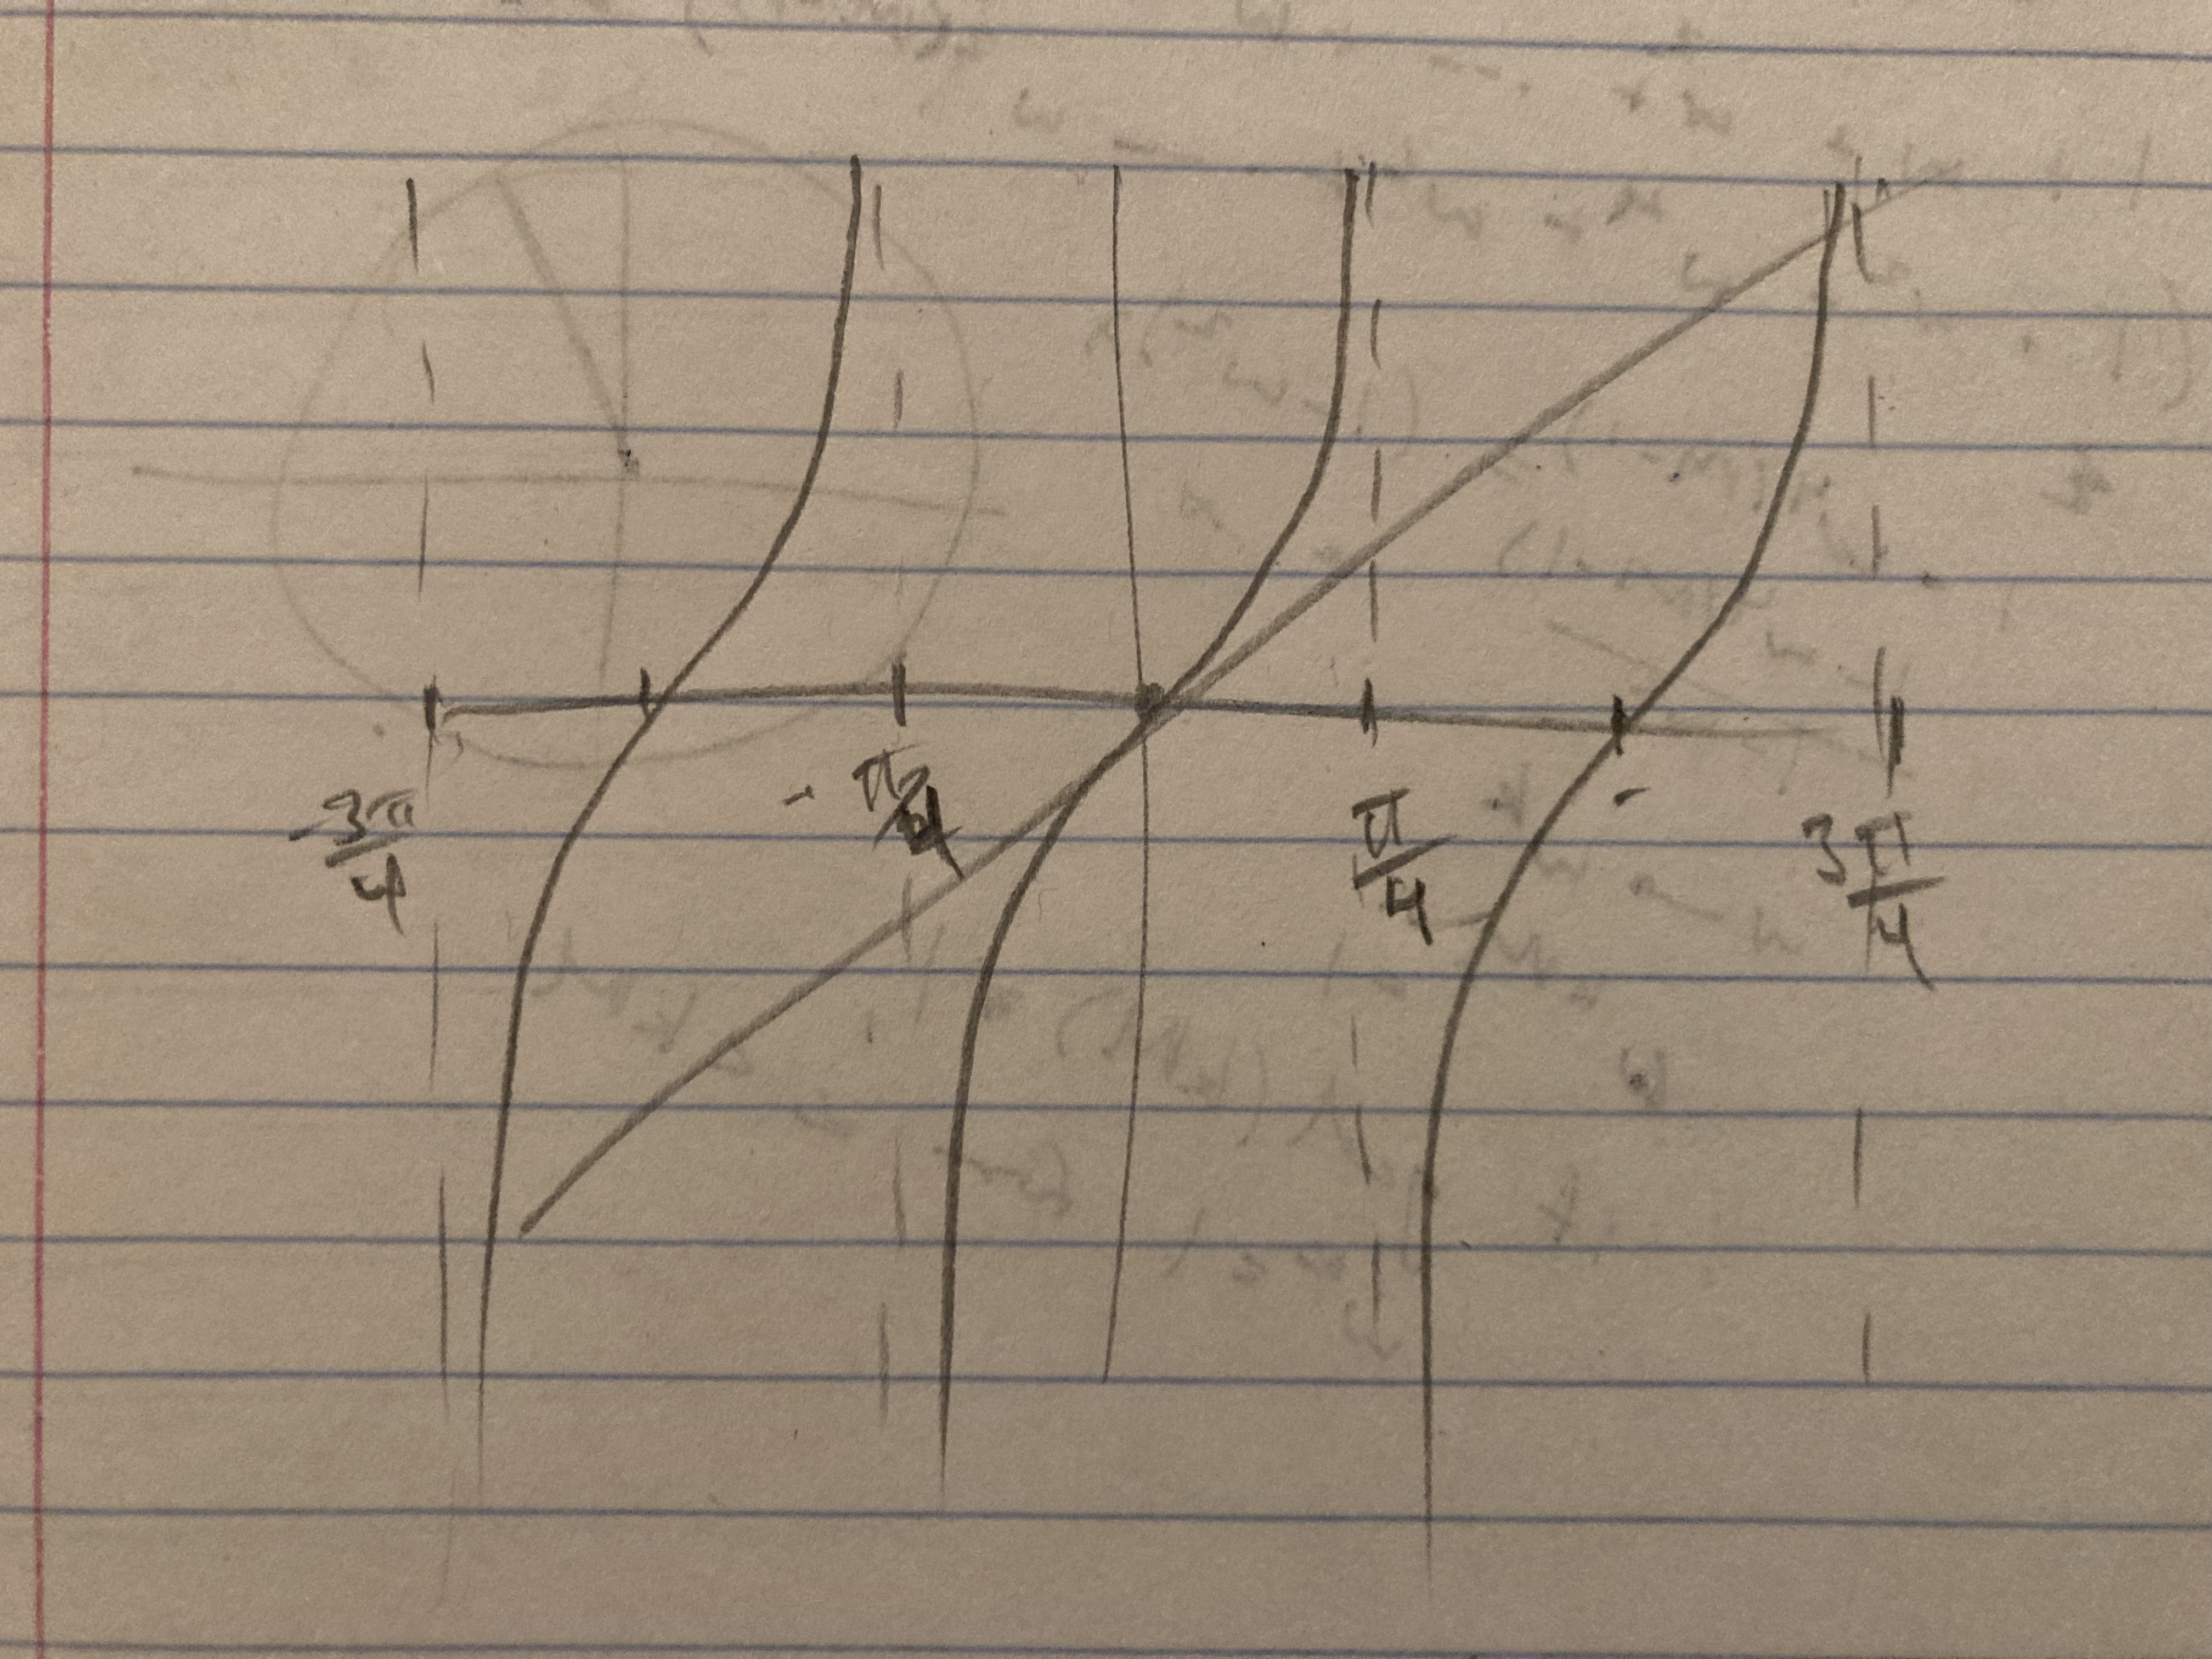
\includegraphics[scale=0.05]{x_and_tanx.jpg}
            \end{center}

        \item [(b)] Use the Bisection method to find an approximation to within $10^{-5}$ to the first positive value of $x$ with $x = \tan{x}$. 
        \begin{answer}
            Here is my bisection.m file:
            \inputminted{matlab}{bisection.m}
            And my function:
            \inputminted{matlab}{myfunc2.m}
            And the script that is ran:
            \inputminted{matlab}{script.m}
            The output given is $x = 0.015625$.
        \end{answer}
    \end{itemize}

\textbf{Exercise 20}:
    Let $f(x) = (x - 1)^{10}, p = 1, $ and $p_{n} = 1 + 1 / n$. Show that $\lvert f(p_{n}) \rvert < 10^{-3}$ whenever $n > 1$ but that $\lvert p - p_{n} \rvert < 10^{-3}$ requires that $n > 1000$.
        \begin{answer}
            We have that $f(p_{n}) = 1 / n^{10} = n^{-10}$. Since $n > 1$, $n^{10} > n^{3}$ and therefore, $n^{-3} > n^{-10}$. So $\lvert f(p_{n}) \rvert = n^{-10} < 10^{-3}$. Now we want to see when 
                \begin{equation*}
                    \lvert 1 / n \rvert < 10^{-3}
                \end{equation*}
            This is true when
                \begin{equation*}
                    1 / n < 10^{-3} \text{ or } -1 / n > 10^{-3}
                \end{equation*}
            This gives:
                \begin{equation*}
                    1 / 10^{-3} < n \text{ or } -1 / 10^{-3} > n
                \end{equation*}
            so:
                \begin{equation*}
                    n > 1000 \text{ or } n < -1000
                \end{equation*}

        \end{answer}

\end{document}
